% Created 2015-05-21 Thu 02:35
\documentclass[a4paper]{article}
\usepackage[utf8]{inputenc}
\usepackage[T1]{fontenc}
\usepackage{fixltx2e}
\usepackage{graphicx}
\usepackage{longtable}
\usepackage{float}
\usepackage{wrapfig}
\usepackage{rotating}
\usepackage[normalem]{ulem}
\usepackage{amsmath}
\usepackage{textcomp}
\usepackage{marvosym}
\usepackage{wasysym}
\usepackage{amssymb}
\usepackage{capt-of}
\usepackage{hyperref}
\tolerance=1000
\usepackage[utf8]{inputenc}
\usepackage[usenames,dvipsnames]{color}
\usepackage{commath}
\usepackage{tikz}
\usetikzlibrary{shapes,backgrounds}
\usepackage{marginnote}
\usepackage{listings}
\usepackage{color}
\usepackage{enumerate}
\hypersetup{urlcolor=blue}
\hypersetup{colorlinks,urlcolor=blue}
\setlength{\parskip}{16pt plus 2pt minus 2pt}
\definecolor{codebg}{rgb}{0.96,0.99,0.8}
\definecolor{codestr}{rgb}{0.46,0.09,0.2}
\DeclareMathOperator{\Dom}{Dom}
\allowdisplaybreaks[4]
\author{Oleg Sivokon}
\date{\textit{<2015-04-03 Fri>}}
\title{Assignment 14, Infinitesimal Calculus}
\hypersetup{
 pdfauthor={Oleg Sivokon},
 pdftitle={Assignment 14, Infinitesimal Calculus},
 pdfkeywords={Infinitesimal Calculus, Assignment, Limits of functions},
 pdfsubject={Fourth asssignment in the course Infinitesimal Calculus},
 pdfcreator={Emacs 25.0.50.1 (Org mode 8.3beta)}, 
 pdflang={English}}
\begin{document}

\maketitle
\tableofcontents

\definecolor{codebg}{rgb}{0.96,0.99,0.8}
\lstnewenvironment{maxima}{%
  \lstset{backgroundcolor=\color{codebg},
    escapeinside={(*@}{@*)},
    aboveskip=20pt,
    showstringspaces=false,
    frame=single,
    framerule=0pt,
    basicstyle=\ttfamily\scriptsize,
    columns=fixed}}{}
}
\makeatletter
\newcommand{\verbatimfont}[1]{\renewcommand{\verbatim@font}{\ttfamily#1}}
\makeatother
\verbatimfont{\small}%
\clearpage

\section{Problems}
\label{sec:orgheadline22}

\subsection{Problem 1}
\label{sec:orgheadline3}
\begin{enumerate}
\item Find the domain of \(f\) defined as \(f(x) = \sqrt{\tan x - 1}\).
\item Find all values of \(x\) in segment \([0, \pi]\), for which \(\abs{\tan x} \leq \sin 2x}\).
\end{enumerate}

\subsubsection{Answer 1}
\label{sec:orgheadline1}
\(\tan x > 1\) where \(\frac{\pi}{4} < x \bmod \frac{\pi}{2} < \frac{\pi}{2}\).
Since we assume that \(f\) is real-valued, we cannot extract roots from negative numbers.

Hence \(\Dom(f) = \{x \in \mathbb{R} \; | \; \frac{\pi}{4} < x \bmod \frac{\pi}{2}
    < \frac{\pi}{2}\}\).

\begin{maxima}
programmode: false;
print (plot2d (tan(x),
    [x, -2 * %pi, 2 * %pi], [y, -3, 3],
    [gnuplot_pdf_term_command, 
     "set term cairolatex standalone pdf size 16cm,10.5cm"],
    [gnuplot_postamble,
     "set arrow from pi/4,-3 to pi/4,3 nohead
      set arrow from pi*5/4,-3 to pi*5/4,3 nohead
      set arrow from -2*pi,1 to 2*pi,1 nohead"],
    [ytics, 1, 1, 1], [xtics, 0, 1, 0],
    [label, ["${\\displaystyle \\frac{\\pi}{4}}$", 1.4, 2.4],
            ["${\\displaystyle \\frac{5\\pi}{4}}$", 3.2, 2.4]],
    [title, "Tangent curve"], [pdf_file, %out]));
(*@\label{orgsrcblock1}
@*)
\end{maxima}

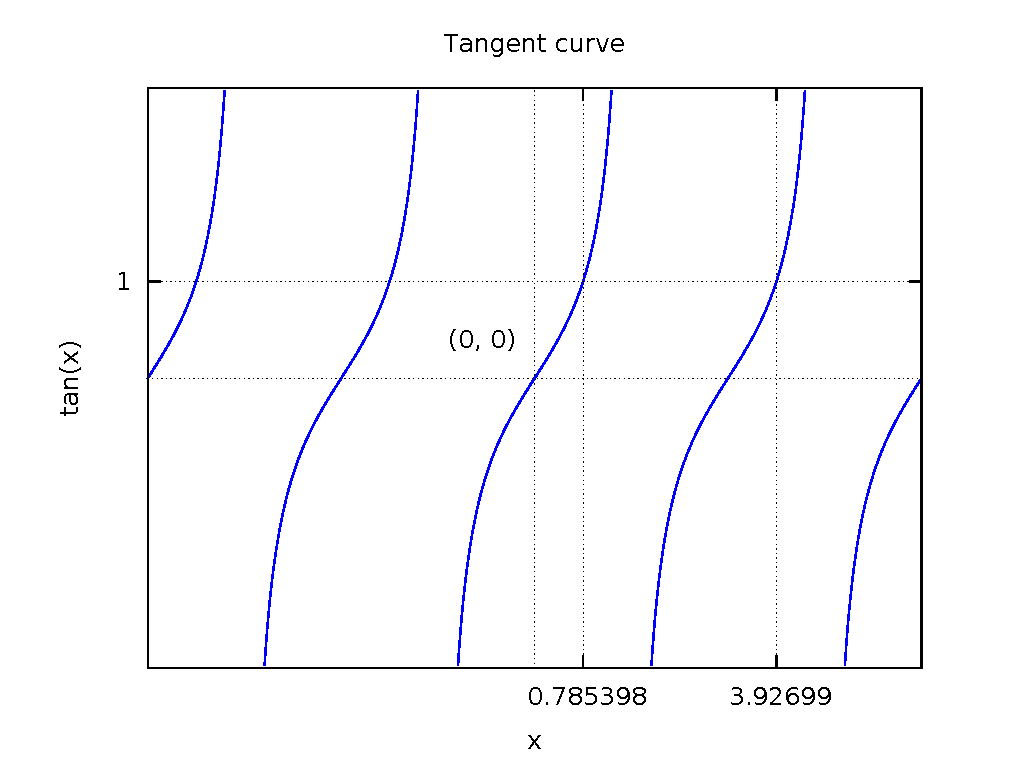
\includegraphics[width=0.9\textwidth]{/home/wvxvw/Documents/uni/infinitesimal-calculus/images/tangent_x.pdf}

\subsubsection{Answer 2}
\label{sec:orgheadline2}
Both functions attain the same values at 0 and \(\frac{\pi}{4}\).  But sine is
a concave function and tanget is a convex function, thus tangent must be less
than sine at this interval.  Tangent keeps increasing until \(\frac{\pi}{2}\),
while sine will be decreasing until \(\frac{3\pi}{2}\), thus, on this interval
tangent is greater than sine.  The functions meet again at \(x=\pi\).

\begin{maxima}
programmode: false;
gnuplot_pdf_command: %command;
print(plot2d ([abs(tan(x)), sin(2 * x)],
    [x, -2 * %pi, 2 * %pi], [y, -1.5, 3],
    [gnuplot_pdf_term_command, 
     "set term cairolatex standalone pdf size 16cm,10.5cm"],
    [gnuplot_postamble,
     "set arrow from pi/4,-1.5 to pi/4,3 nohead
      set arrow from pi,-1.5 to pi,3 nohead
      set arrow from -2*pi,1 to 2*pi,1 nohead
      set key spacing 1.8 left bottom"],
    [xtics, 0, 1, 0], [ytics, 1, 1, 1],
    [label, ["${\\displaystyle \\frac{\\pi}{4}}$", 1.4, 2.1],
            ["${\\displaystyle \\pi}$", 3.4, 2.1]],
    [title, "Tangent curve intersecting with sine curve"],
    [pdf_file, %out]));
(*@\label{orgsrcblock2}
@*)
\end{maxima}

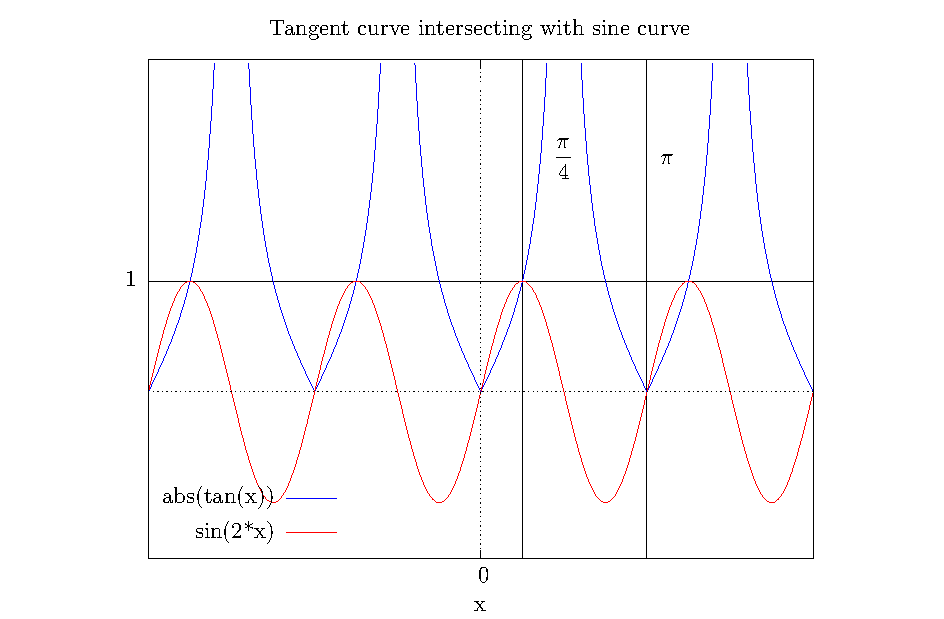
\includegraphics[width=0.9\textwidth]{/home/wvxvw/Documents/uni/infinitesimal-calculus/images/abstangent_x.pdf}

\subsection{Problem 2}
\label{sec:orgheadline9}
Let \(f\), \(g\) and \(h\) be functions from \(\mathbb{R}\) to \(\mathbb{R}\).
\begin{enumerate}
\item If \(f \circ g = f \circ h\), does it follow \(g = h\)?
\item If \(f \circ g = f \circ h\), and \(f\) is one-to-one, does it follow \(g = h\)?
\item If \(f \circ g = f \circ h\), and \(f\) is onto, does it follow \(g = h\)?
\item If \(f \circ g\) is increasing, and \(f\) is decreasing, does it follow that
\(g\) is increasing?
\item If \(f \circ g\) is increasing, and \(f\) is one-to-one, does it follow that
\(g\) is monotonic?
\end{enumerate}

\subsubsection{Answer 3}
\label{sec:orgheadline4}
No, \(g\) and \(h\) are not necessarily equal.  Whenever co-domain of \(f\)
doesn't contain some real number, \(g\) and \(h\) may differ in that input.
For example, let \(f(x) = 2x\), \(g(x) = (x \bmod 2) + x\) and
\(h(x) = (x \bmod 2) * 2 + x\).  Because \(f\) in this example will only
generate even numbers, the \((x \bmod 2)\) term will always be zero,
thus \(f \circ g = f \circ h\), but, obviously, \(g \neq h\).

\subsubsection{Answer 4}
\label{sec:orgheadline5}
No, it isn't sufficient for \(f\) to be one-to-one to ensure right-cancellation
property under composition.  The example given in \ref{sec:orgheadline4} is applicable
in this case too since whenever \(f(x) = f(y)\) so is \(x = y\) (since multiplication
does have the cancellation property).

\subsubsection{Answer 5}
\label{sec:orgheadline6}
Yes, if \(f\) is onto, then the composition is right-cancellable.  Suppose,
for contradiction it wasn't, then for some \(y\) \(g(y) \neq h(y)\), but
\(y = f(x)\) (since by definition of a total function, every element in
its co-domain has an element in its domain).  Hence \(g(f(x)) \neq h(f(x))\),
but we are given that \(g \circ f = h \circ f\), which is a contradiction.
Hence functions are equal.

\subsubsection{Answer 6}
\label{sec:orgheadline7}
No, \(g\) doesn't need to be increasing.  Put \(g(x) = f(x) = -x\), both \(f\)
and \(g\) are decreasing but \(f \circ g = Id\), which is an increasing function.

\subsubsection{Anser 7}
\label{sec:orgheadline8}
No, \(g\) is not necessarily monotonic.  Put \(f(x) = x(-1)^x\) and \(g(x) = \abs{x}\).
Then \((f \circ g)(x) = \abs{x(-1)^x} = x\abs{(-1)^x} = x\).  \(f \circ g\) is
increasing, \(f\) is one-to-one, but \(g\) isn't monotonic: it decreases whenever
\(x\) is negative and increases whenever \(x\) is positive.

\subsection{Problem 3}
\label{sec:orgheadline12}
\begin{enumerate}
\item Prove from \(\epsilon-\delta\) definition of limit that 
\(\lim_{x \to 2}\sqrt{3x - 2} = 2\).
\item Prove from \(\epsilon-M\) definition of limit that 
\(\lim_{x \to \infty}\frac{x}{x+\sin x} = 1\).
\end{enumerate}

\subsubsection{Answer 8}
\label{sec:orgheadline10}
Recall the definition:
\begin{quote}
For all \(\epsilon > 0\) there exists \(\sigma > 0\) s.t. for all \(x\) in
\(\Dom(f(x))\) which satisfy \(0 < \abs{x - x_0} < \sigma\) the inequality
\(\abs{f(x) - L} < \epsilon\) holds.
\end{quote}

Let \(\epsilon\) be arbitrary real, put
\begin{equation*}
  \begin{aligned}
      &\abs{f(x) - L}          &< \epsilon                         &\iff \\
      &\abs{\sqrt{3x - 2} - 2} &< \epsilon                               \\
      &\textit{Suppose $\sqrt{3x - 2} - 2 > 0$}                          \\
    0 &< \sqrt{3x - 2} - 2     &< \epsilon                         &\iff \\
    0 &< \sqrt{3x - 2}         &< \epsilon + 2                     &\iff \\
    0 &< 3x - 2                &< (\epsilon + 2)^2                 &\iff \\
    0 &< 3x - 2                &< \epsilon^2 + 4\epsilon + 4       &\iff \\
    0 &< 3x - 6                &< \epsilon^2 + 4\epsilon           &\iff \\
    0 &< x - 2                 &< \frac{\epsilon^2 + 4\epsilon}{3}       \\
      &\textit{Similarly for $\sqrt{3x - 2} - 2 < 0$}                    \\
    0 &> \sqrt{3x - 2} - 2     &> -\epsilon                        &\iff \\
    0 &> \sqrt{3x - 2}         &> -\epsilon + 2                    &\iff \\
    0 &> 3x - 2                &> (-\epsilon + 2)^2                &\iff \\
    0 &> 3x - 2                &> \epsilon^2 - 4\epsilon + 4       &\iff \\
    0 &> 3x - 6                &> \epsilon^2 - 4\epsilon           &\iff \\
    0 &> x - 2                 &> \frac{\epsilon^2 - 4\epsilon}{3}
  \end{aligned}
\end{equation*}

Hence, we can choose \(\delta\) to be \(\frac{\epsilon^2 - 4\epsilon}{3}\)
whenever \(x < x_0\) and \(\frac{\epsilon^2 + 4\epsilon}{3}\) whenever
\(x > x_0\), which completes the proof.

\subsubsection{Answer 9}
\label{sec:orgheadline11}
Recall the definition:
\begin{quote}
For all \(\epsilon > 0\) there exists \(M > 0\) s.t. for all \(x\) in
\(\Dom(f(x))\) \(x > M\) implies \(\abs{f(x) - L} < \epsilon\).
\end{quote}

Let \(\epsilon > 0\), then look for appropriate value for \(x\):
\begin{align*}
  &\abs{\frac{x}{x + \sin x} - 1}                   &< \epsilon &\iff \\
  &\abs{\frac{x}{x + \sin x} - \sin^2 x - \cos^2 x} &< \epsilon &\iff \\
  &\abs{\frac{x - \sin^2 x(x + \sin x) -
      \cos^2 x(x + \sin x)}{x + \sin x}}            &< \epsilon &\iff \\
  &\abs{\frac{x - x\sin^2 x - \sin^3 x -
      x\cos^2 x - \cos^2 x \sin x}{x + \sin x}}     &< \epsilon &\iff \\
  &\abs{\frac{x(1 - \sin^2 - \cos^2 x) -
      \sin x(\sin^2 x - \cos^2)}{x + \sin x}}       &< \epsilon &\iff \\
  &\abs{\frac{x(1 - 1) - \sin x(1)}{x + \sin x}}    &< \epsilon &\iff \\
  &\abs{\frac{-\sin x}{x + \sin x}}                 &< \epsilon \\
\end{align*}

Assume \(x > 0\):
\begin{align*}
  &\frac{-\sin x}{x + \sin x} &< \epsilon &\iff \\
  &-\sin x                    &< \epsilon(x + \sin x) &\iff \\
  &-\sin x                    &< \epsilon x + \epsilon \sin x &\iff \\
  &-\epsilon x                &< \sin x + \epsilon \sin x &\iff \\
  &-x                         &< \frac{\sin x + \epsilon \sin x}{\epsilon} &\iff \\
  &x                          &> \frac{\sin x(1 + \epsilon)}{\epsilon}
\end{align*}

Put \(M = \max\left(0, \frac{\sin x(1 + \epsilon)}{\epsilon}\right)\). If \(x > M\), then
\(x > 0\) and \(x > \frac{\sin x(1 + \epsilon)}{\epsilon}\), hence:
\begin{align*}
  &x                              &> \frac{\sin x(1 + \epsilon)}{\epsilon} \\
  &\hdots \textit{Reverse the calculations above} \\
  &\frac{-\sin x}{x + \sin x}     &< \epsilon \\
  &\hdots \\
  &\abs{\frac{x}{x + \sin x} - 1} &< \epsilon.
\end{align*}

Which completes the proof.

\subsection{Problem 4}
\label{sec:orgheadline15}
\begin{enumerate}
\item Let \(f\) be a function defined in the neighborhood of \(x_0\).
Express ``\(f\) doesn't have a limit at \(x_0\)'' using:
\begin{itemize}
\item \(\epsilon-\sigma\) language.
\item Using Heine definition of limit (for sequences).
\end{itemize}

\item Prove that \(f(x) = \frac{x}{x - \lfloor x \rfloor}\) doesn't have
a finite limit at \(x \to 0\) in the following ways:
\begin{itemize}
\item By using \(\epsilon-\sigma\) definition given above.
\item By using Heine definition of limit (also given above).
\end{itemize}
\end{enumerate}

\subsubsection{Answer 10}
\label{sec:orgheadline13}
Recall the \(\epsilon-\delta\) definition:

\emph{The limit of $f(x)$ at $x_0$ is defined to be $L$ s.t. for every
  $\epsilon > \abs{f(x) - L} > 0$ we can find $\delta > \abs{x - x_0} >
  0$.}

To negate this is to say that there exists such \(\epsilon\) for which
we can't find a positive \(\delta\) larger than the distance from \(x\) to
\(x_0\).

\emph{Heine defines limit to be $L$ whenever for every sequence $(x_n)$ which
  convergest to $x_0$, every sequence of function values $f(x_n)$ converges
  to $L$.}

To negate this definition we claim that there exists a sequence \((x_m)\),
which convergest to \(x_0\), however \(f(x_m)\) doesn't converge to \(L\).

\subsubsection{Answer 11}
\label{sec:orgheadline14}
I'll do the Heine first, because it's easier.  We can choose sequences
\((x_n) = -\frac{\pi}{2nx}\) and \((x_m) = \frac{\pi}{2mx}\), both are
immediately reducible to the limit of a fraction as \(x\) approaches zero,
hence, the limit for both is zero.  Now, if we plug them back into \(f\), we
get:

\begin{align*}
  \lim_{x \to 0}\frac{x}{x - \lfloor \sin x \rfloor}
  &= \lim_{x \to 0}\frac{x}{x - 0} \\
  &\textit{$\lfloor \sin x \rfloor = 0$ whenever $0 < x < \frac{\pi}{2}$} \\
  &= 1\;.
\end{align*}

Similarly:

\begin{align*}
  \lim_{x \to 0}\frac{x}{x - \lfloor \sin x \rfloor} 
  &= \lim_{x \to 0}\frac{x}{x + 1} \\
  &\textit{$\lfloor \sin x \rfloor = -1$ whenever $0 > x > -\frac{\pi}{2}$} \\ 
  &= 0\;.
\end{align*}

Now, the \(\epsilon-\sigma\) approach:

Since we can pick arbitrary \(\epsilon\), put \(\epsilon = \frac{1}{2}\). Now, we
could try to find the limit withing \(\pi\) distance from zero.  Assuming thus
\(x \in (\pi, -\pi)\).

\begin{align*}
  -&\frac{1}{2}
  < \frac{\sigma}{\sigma - \lfloor \sin \sigma \rfloor} - L
  < \frac{1}{2} \\
  -&\frac{1}{2} < \frac{\sigma}{\sigma - 0} - L < \frac{1}{2} \\
  -&\frac{1}{2} < 1 - L < \frac{1}{2} \\
  -&\frac{3}{2} < -L < -\frac{1}{2} \\
   &\frac{3}{2} > L > \frac{1}{2} \\
   &\textit{Similarly:} \\
  -&\frac{1}{2}
  < \frac{-\sigma}{\lfloor - \sin \sigma \rfloor -\sigma} - L
  < \frac{1}{2}\\
  -&\frac{1}{2} < \frac{-\sigma}{-\sigma + 1} - L < \frac{1}{2} \\
  -&\frac{1}{2} - \frac{-\sigma}{-\sigma + 1} < -L
  < \frac{1}{2} - \frac{-\sigma}{-\sigma + 1} \\
  -&\frac{-\sigma + 1 + 2\sigma}{-2\sigma + 2}
  < -L < \frac{1}{2} - \frac{-\sigma}{1 - \sigma} \\
  -&\frac{1 + \sigma}{-2\sigma + 2} < -L
  < \frac{1}{2} - \frac{-\sigma}{1 - \sigma} \\
   &\frac{-1 - \sigma}{-2\sigma + 2} < -L
  < \frac{1}{2} - \frac{-\sigma}{1 - \sigma} \\
   &\frac{-1(1 + \sigma)}{-1(2\sigma - 2)} < -L
  < \frac{1}{2} - \frac{-\sigma}{1 - \sigma} \\
   &\frac{1 + \sigma}{2\sigma - 2} < -L
  < \frac{1}{2} - \frac{-\sigma}{1 - \sigma} \\
   &\textit{Since $\sigma > 0$} \\
   &\frac{1 + \sigma}{2\sigma + 2} < -L
  < \frac{1}{2} - \frac{-\sigma}{1 - \sigma} \\
   &\frac{1}{2} < -L < \frac{1}{2} - \frac{-\sigma}{1 - \sigma} \\
   &\textit{Contradiction: $L > \frac{1}{2}$ and $L < \frac{1}{2}$.}
\end{align*}

\begin{maxima}
programmode: false;
gnuplot_pdf_command: %command;
print(plot2d (x / (x - floor(sin(x))),
    [x, -2 * %pi, 2 * %pi], [y, -2, 2],
    [gnuplot_pdf_term_command, 
     "set term cairolatex standalone pdf size 16cm,10.5cm"],
    [ylabel, "${\\displaystyle \\frac{x}{x - \\lfloor \\sin x \\rfloor}}$"],
    [title, concat("${\\displaystyle \\lim_{x \\to 0}",
               "\\frac{x}{x - \\lfloor \\sin x \\rfloor}}$")],
    [pdf_file, %out]));
(*@\label{orgsrcblock3}
@*)
\end{maxima}

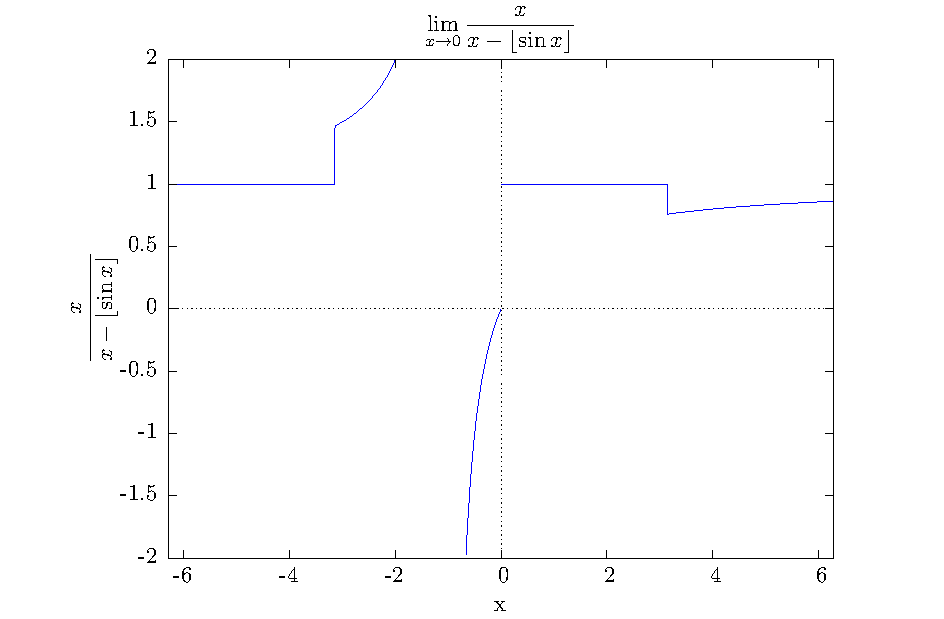
\includegraphics[width=.9\linewidth]{/home/wvxvw/Documents/uni/infinitesimal-calculus/images/nolimit.pdf}


\subsection{Problem 5}
\label{sec:orgheadline21}
Find limits of:
\begin{enumerate}
\item \(\lim_{x \to 0}\frac{1 - \cos x}{x \sin x}\).
\item \(\lim_{x \to 0}\frac{x + 7x^3}{x^3 - 2x^4}\).
\item \(\lim_{x \to 0}\frac{x^2 - 1}{2x^3 - x^2 - x}\).
\item \(\lim_{x \to 0}(\sqrt{1 + x + x^2} - \sqrt{1 - x + x^2})\).
\item \(\lim_{x \to k}\lfloor x \rfloor \tan \frac{\pi x}{2}\), \(k = 0, 1, 2\).
\end{enumerate}

\subsubsection{Answer 12}
\label{sec:orgheadline16}
\begin{maxima}
tex(limit((1 - cos(x)) / (x * sin(x)), x, 0));
(*@\label{orgsrcblock4}
@*)
\end{maxima}

\({{1}\over{2}}\)

\textbf{Proof:}
\begin{align*}
  \lim_{x \to 0}\frac{1 - \cos x}{x \sin x} &= 
  \lim_{x \to 0}\frac{(1 - \cos x) * (1 + \cos x)}{x \sin x (1 + \cos x)} \\
  &= \lim_{x \to 0}\frac{1 - \cos^2 x}{x \sin x (1 + \cos x)} \\
  &= \lim_{x \to 0}\frac{\sin^2 x}{x \sin x (1 + \cos x)} \\
  &= \lim_{x \to 0}\frac{\sin x}{x (1 + \cos x)} \\
  &= \lim_{x \to 0}\frac{\sin x}{x} * \lim_{x \to 0}\frac{1}{1 + \cos x} \\
  &= 1 * \lim_{x \to 0}\frac{1}{1 + \cos x} \\
  &= \lim_{x \to 0}\frac{1}{1 + 1} \\
  &= \frac{1}{2}
\end{align*}

\subsubsection{Answer 13}
\label{sec:orgheadline17}
\begin{maxima}
tex(limit((x + 7 * x^3) / (x^3 - 2 * x^4), x, 0));
(*@\label{orgsrcblock5}
@*)
\end{maxima}

\(\infty\)

\textbf{Proof:}
\begin{align*}
  \lim_{x \to 0}\frac{x + 7x^3}{x^3 - 2x^4} &= 
  \lim_{x \to 0}\frac{1 + 7x^2}{x^2 - 2x^3} \\
  &= \lim_{x \to 0}\frac{1 - 4x^2}{x^2 - 2x^3} + \frac{11x^2}{x^2 - 2x^3} \\
  &= \lim_{x \to 0}\frac{(1 - 2x)(1 + 2x)}{x^2(1 - 2x)} + \frac{11}{1 + 2x} \\
  &= \lim_{x \to 0}\frac{1 + 2x}{x^2} + \frac{11}{1 + 2x} \\
  &= \lim_{x \to 0}\frac{1}{x^2} + \frac{2x}{x^2} + \frac{11}{1 + 2x} \\
  &= \lim_{x \to 0}\frac{1}{x^2} + \frac{2}{x} + \frac{11}{1 + 2x} \\
  &= \lim_{x \to 0}\frac{1}{x^2} + \lim_{x \to 0}\frac{2}{x} + \lim_{x \to 0}\frac{11}{1 + 2x} \\
  &= \infty + \infty + 11 & \textit{Using ifinite limits addition} \\
  &= \infty
\end{align*}

\subsubsection{Answer 14}
\label{sec:orgheadline18}
\begin{maxima}
tex(limit((x^2 - 1) / (2 * x^3 - x^2 - x), x, 0));
(*@\label{orgsrcblock6}
@*)
\end{maxima}

\({\it infinity}\)

\textbf{Proof:}
\begin{align*}
  \lim_{x \to 0}\frac{x^2 - 1}{2x^3 - x^2 - x} &=
  \lim_{x \to 0}\frac{(x - 1)(x + 1)}{x^2(x - 1) + x(x^2 - 1)} \\
  &= \lim_{x \to 0}\frac{(x - 1)(x + 1)}{x^2(x - 1) + x(x - 1)(x + 1)} \\
  &= \lim_{x \to 0}\frac{(x - 1)(x + 1)}{(x - 1)(x^2 + x(x + 1))} \\
  &= \lim_{x \to 0}\frac{x + 1}{x^2 + x(x + 1)} \\
  &= \lim_{x \to 0}\frac{x + 1}{x^2 + x^2 + x} \\
  &= \lim_{x \to 0}\frac{x + 1}{2x^2 + x} \\
  &= \lim_{x \to 0}\frac{x + 1}{x(2x + 1)} \\
  &= \lim_{x \to 0}\frac{x + 1}{x} * \lim_{x \to 0}\frac{1}{2x + 1} \\
  &= \lim_{x \to 0}\frac{x + 1}{x} * 1 \\
  &= \infty
\end{align*}

\subsubsection{Answer 15}
\label{sec:orgheadline19}
\begin{maxima}
tex(limit(sqrt(1 + x + x^2) - sqrt(1 - x + x^2), x, 0));
(*@\label{orgsrcblock7}
@*)
\end{maxima}

\(0\)

\textbf{Proof:} this function is continuous at \(x = 0\) since square root
is continuous at 1 and this function is offset by one.  From definition
of continuity we know that the limit of the function coincides with its
value, hence the limit is \(\sqrt{1 + 0 + 0^2} - \sqrt{1 - 0 + 0^2} = 1 - 1 = 0\).

\subsubsection{Answer 16}
\label{sec:orgheadline20}
\begin{maxima}
for i : 0 thru 2 do
    tex(limit(floor(x) * tan((%pi * x) / 2), x, i));
(*@\label{orgsrcblock8}
@*)
\end{maxima}

\(0\)
\({\it und}\)
\(0\)
\end{document}